 \documentclass[a4paper,11pt]{article}
% \documentclass{svjour3}
\usepackage[latin1]{inputenc}
\usepackage{epsfig}
\usepackage{listings,xcolor}
\usepackage{graphicx}
\usepackage{url}
\usepackage{float}
\usepackage{stmaryrd}
\usepackage{ifpdf}
\usepackage{tikz}
\usetikzlibrary{shapes.geometric, arrows}

\lstdefinestyle{Common} {
    extendedchars=\true,
    language={Prolog},
    %%frame=single,
    %%rulecolor=\color{black}
    framesep=3pt,%expand outward.
    framerule=0.4pt,%expand outward.
    xleftmargin=6pt,%make the frame fits in the text area.
    xrightmargin=3.4pt,%make the frame fits in the text area.
}

\lstdefinestyle{A}
{
    style=Common,
    basicstyle=\color{black}\ttfamily,
    keywordstyle=\color{gray},
    identifierstyle=\color{blue},
    stringstyle=\color{darkgray},
    commentstyle=\color{darkgray}
}

\newcommand{\Author}{H\'ector Castillo}
\newcommand{\Title}{Market Power ABM}


\hypersetup{colorlinks=false}

\ifpdf\hypersetup{
    pdftitle = {\Title},%
    pdfsubject = {\Title},%
    pdfkeywords = {stochastic logic programs, UPV },
    pdfauthor = {\textcopyright\ \Author},
    pdfcreator = {\LaTeX},
    pdfproducer = {pdfeTeX-0.\the\pdftexversion\pdftexrevision}
   }
\pdfinfo{/CreationDate (\today)}
\fi

\pagestyle{plain}


% \floatstyle{boxed}
\newfloat{program}{h}{lop}
\floatname{program}{Example}

\newbox\examplebox
\newenvironment{example}[2]{%
    \program
    \caption{#2}%
    \label{#1}%
    \verbatim
}{%
    \endverbatim
    \vskip-.7\baselineskip
    \endprogram
}



\begin{document}

\title{\Title}
\author{\Author}
\maketitle


\section{Introduction}
With the intention of obtaining a framework that allows to execute ABM in Python, we present \texttt{market\_power}, with the next elements:

\begin{itemize}

\item Auxiliary files:
    \begin{itemize}
	  \item  \texttt{requirements.txt}: list of the necessary python packages
	  \item  \texttt{util/statistics.py}: class for managing the output 
	  \item  \texttt{util/stats\_array.py}: it contains the code to plot with pyplot, bokeh, grace and gretl. 
	  \item  \texttt{util/log.py}: class for managing the logging
	  \item  \texttt{output/*}: the files generated (plots mainly)
	  \item  \texttt{test/*}: unit tests
    \end{itemize}
\end{itemize}


\pagebreak



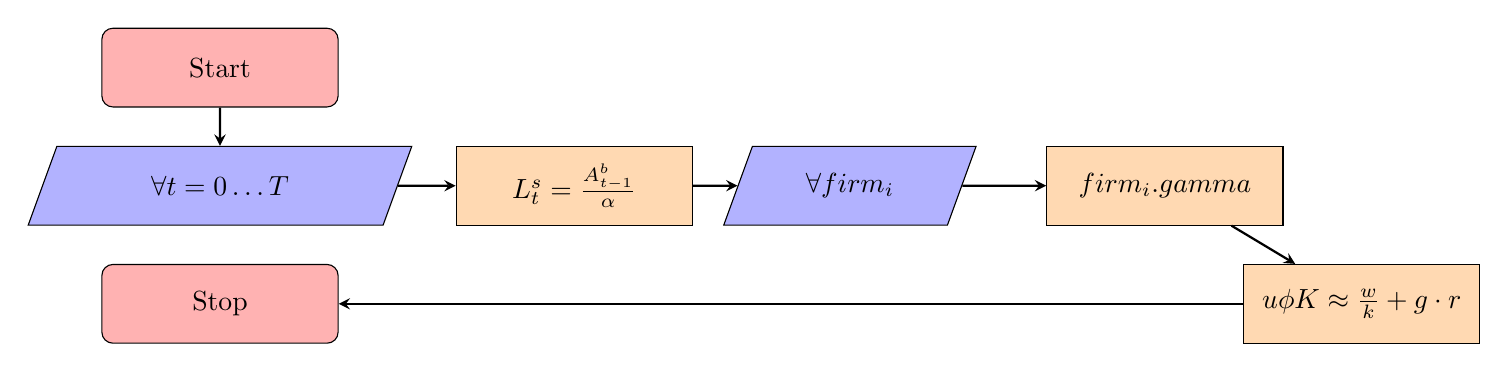
\begin{tikzpicture}[node distance=1.5cm]
      \tikzstyle{startstop} = [rectangle, rounded corners, minimum width=3cm, minimum height=1cm,text centered, draw=black, fill=red!30]
      \tikzstyle{io} = [trapezium, trapezium left angle=70, trapezium right angle=110, minimum width=3cm, minimum height=1cm, text centered, draw=black, fill=blue!30]
      \tikzstyle{process} = [rectangle, minimum width=3cm, minimum height=1cm, text centered, draw=black, fill=orange!30]
      \tikzstyle{decision} = [diamond, minimum width=3cm, minimum height=1cm, text centered, draw=black, fill=green!30]
      \tikzstyle{arrow} = [thick,->,>=stealth]

      \node (start) [startstop, xshift=-3cm] {Start};
      \node (in1) [io, below of=start] { $ \forall t=0 \dots T $ };
      \draw [arrow] (start) -- (in1);
      \node (pro1) [process, right of=in1, xshift=3cm] {   $ L_{t}^{s}=\frac{   A_{t-1}^{b} }{\alpha } $  };
      \draw [arrow] (in1) -- (pro1);
      \node (in2) [io, right of=pro1, xshift=2cm] { $ \forall firm_{i} $ };
      \draw [arrow] (pro1) -- (in2);
      \node (pro2) [process, right of=in2, xshift=2.5cm] {   $ firm_{i}.gamma $  };
      \draw [arrow] (in2) -- (pro2);
      \node (pro3) [process, below of=pro2, xshift=2.5cm] { $u \phi K \approx \frac{w}{k}+g \cdot  r$ };
      \draw [arrow] (pro2) -- (pro3);
      \node (stop) [startstop, below of=in1] {Stop};
      \draw [arrow] (pro3) -- (stop);

\end{tikzpicture}


\end{document}
